\section{Empresa vs. Mercado}
\begin{figure}
    \centering
    % \includegraphics[width=8cm]{./Clases/figs/}
\end{figure}

\subsection{Procedimiento}
\begin{itemize}
    \item Inciso:
        \begin{center}
            \begin{figure}[!htb]
                \centering
                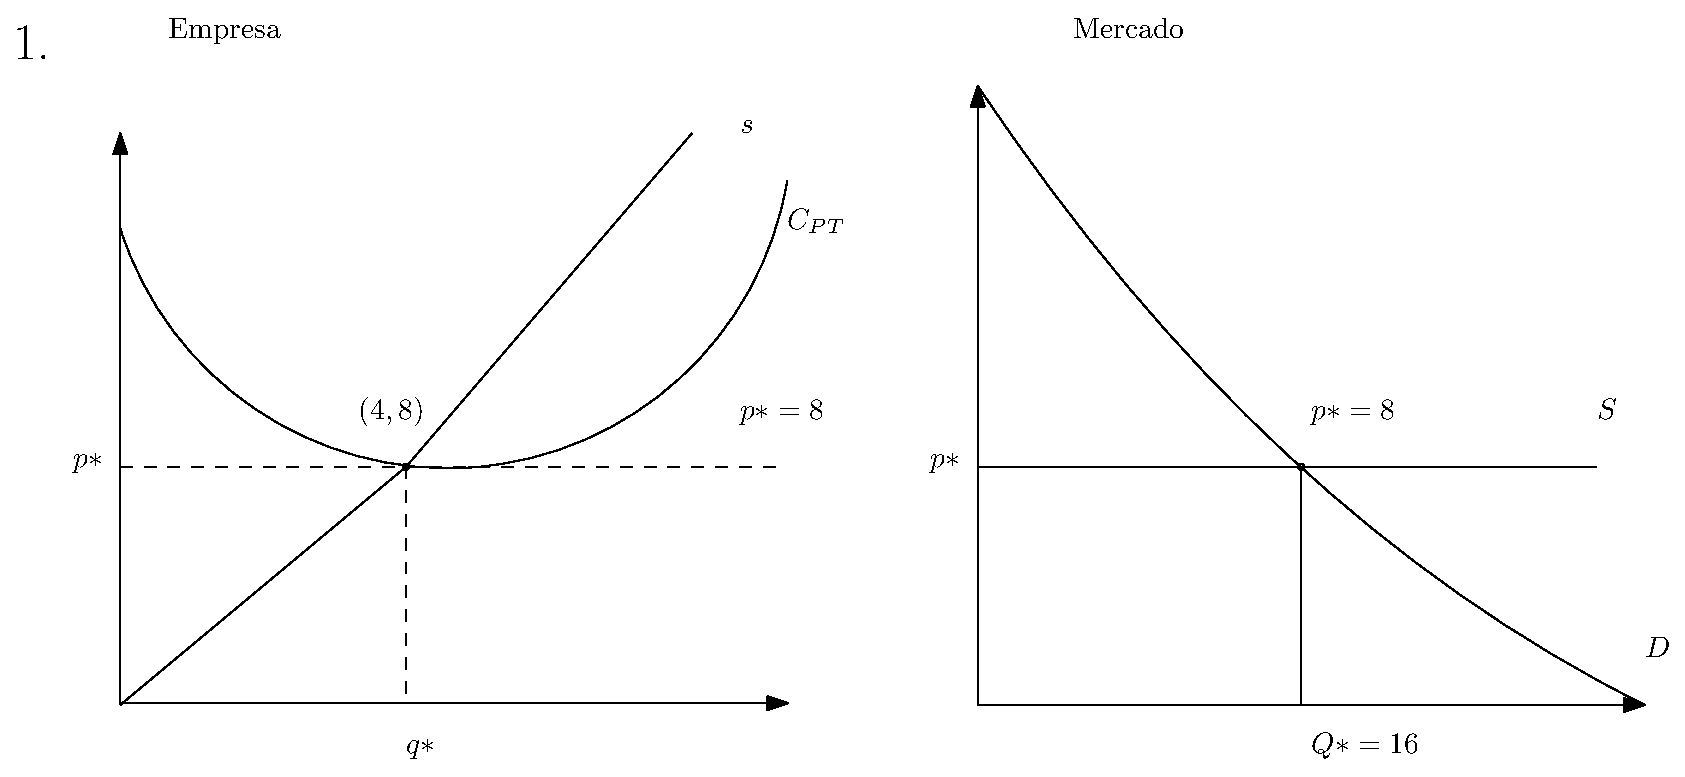
\includegraphics[width=18cm]{./Clases/figs/01.eps}
            \end{figure}
        \end{center}
        \begin{itemize}                
        \item Debemos sacar el $p*$ \& $q*$ 
        \end{itemize}
        \begin{center}
           \begin{align*}
               C_T &= 16 + q^2 \\ 
               Q &= 24 - p \\ 
               \text{ Min.  }\; C_{PT}: \\ 
                    \frac{C_T}{q} &= \frac{16+q^2}{q} \\ 
                    \text{ Costo promedio Total }: \qq C_{PT} &= \frac{16}{q} + q \\ 
                    \text{ Derivamos }: \qq   
                        \dervpar{C_{PT}}{q} &= -16q^{-2} + 1 \\  
                        \text{ Igualar a 0 }: \qq  -16q^{-2} + 1 = 0 \qimplies q* = 4 \\ 
                C_{PT}(q*=4) &= \frac{16+(4)^2}{4} = 8 \\  
                \therefore \qq \text{ El precio \&  la cantidad es:  }\; p*&=8, q*=4, Q*=16 \\ 
           \end{align*}
        \end{center}
    
    \item Inciso: 
        \begin{itemize}
            \item Dadas las siguentes funciones: 
                \begin{center}
                    \begin{figure}[!htb]
                        \centering
                        \includegraphics[width=18cm]{./Clases/figs/02.eps}
                    \end{figure}
                \end{center}
                \begin{center}
                   \begin{align*}
                       C_{T} &= 10q^2+10 \qq \qq Q = 1,000-p \\ 
                   \end{align*}
                   \begin{itemize}
                       \item Sacar: $q*$, $Q*$, $p*$ y el número de empresas.  
                   \end{itemize}
                   \begin{align*}
                       C_{TP} &= \frac{10q^2+10}{q} = 10q +\frac{10}{q} \\
                       \dervpar{C_{PT}}{q} &= 10 - 10q^{-2} \qimplies q* = 1 \\  
                       C_{TP}(q*=1) &= 10(1)^1 + \frac{10}{1} = 20 \\ 
                       \therefore \qq C_{TP}&=20 \; \text{ ó }\; p*=20, q*=1 \\   
                   \end{align*}
                \end{center}
        \end{itemize}
\end{itemize}
